Este capítulo describe cómo se prepara un programa en la PC, cómo se envía a
la FPGA y de qué manera se observa el estado del procesador durante su
ejecución. En ese recorrido participan el assembler, la aplicación
\tech{viewrv} y el protocolo de comunicación sobre UART.

\section{Recorrido completo}

El punto de partida es un programa escrito en el lenguaje assembler del TP3.
El assembler traduce sus instrucciones a una imagen de bytes y conserva una
relación entre las direcciones de las instrucciones y las líneas del código
fuente. Con esa información, \tech{viewrv} puede cargar el programa y
relacionar lo que ocurre en el procesador con el texto que escribió el usuario.

La figura~\ref{fig:flujo-completo} muestra el recorrido completo: la PC
prepara y envía la imagen, la FPGA la almacena en IMEM y ejecuta el programa,
y la PC recibe las observaciones para presentarlas al usuario. Una vez
configurada la placa, pueden cargarse programas diferentes sobre el mismo
bitstream.

\begin{figure}[H]
  \centering
  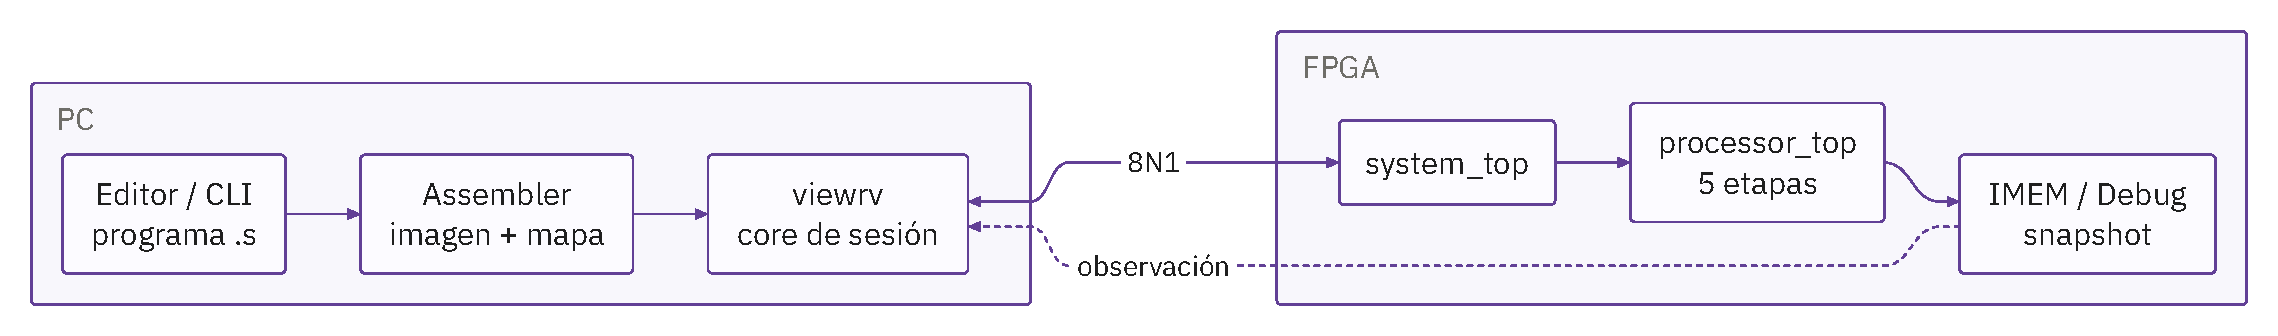
\includegraphics[width=\textwidth]{flujo-completo.pdf}
  \caption{Recorrido desde el programa assembler hasta la ejecución y la
  observación del procesador.}
  \label{fig:flujo-completo}
\end{figure}

\section{El assembler}

El assembler convierte el código fuente en las palabras de instrucción que
entiende el procesador. Cada instrucción ocupa cuatro bytes en orden
little-endian y se incorpora a una imagen continua que comienza en la dirección
cero. Además, el assembler genera un mapa que relaciona la dirección de cada
instrucción con su línea en el programa original.

La aplicación entrega el texto completo mediante la siguiente interfaz:

\begin{codebox}[language=Python]
assemble(source_text: str) -> AssemblyResult
\end{codebox}

El resultado reúne la imagen y el mapa cuando la traducción es correcta, o un
diagnóstico cuando encuentra un error:

\begin{itemize}
  \item \code{image}: los bytes de la imagen, o \code{None} si hubo un error;
  \item \code{pc_to_line}: la relación entre cada PC de instrucción y su línea
  fuente;
  \item \code{error}: un diagnóstico con línea y mensaje, o \code{None}.
\end{itemize}

Para traducir el programa, el assembler comprueba los mnemónicos, operandos,
registros, etiquetas y rangos de inmediatos admitidos por el lenguaje. El mapa
PC-línea queda en la aplicación, mientras que la imagen es el contenido que se
envía a la FPGA.

La traducción y la ejecución comprueban aspectos diferentes. El assembler
determina si el programa puede codificarse; después, la FPGA valida que la
imagen quepa en IMEM y el procesador comprueba las instrucciones y los accesos
durante la ejecución. Por eso, un ensamblado correcto no asegura por sí solo
que el programa termine normalmente.

El assembler está implementado en \code{tp3/software/assembler.py}. Su
interfaz, el lenguaje, la codificación y los diagnósticos se especifican en
\doc{software/assembler_interface.md}{la documentación del assembler}.

\section{\texorpdfstring{\tech{viewrv}}{viewrv}}

\tech{viewrv} es la aplicación local que permite preparar programas, controlar
la placa y observar el procesador. Ofrece una interfaz gráfica para trabajar
con el código y visualizar el pipeline, además de una interfaz de línea de
comandos para operar desde una terminal o automatizar recorridos.

Ambas interfaces utilizan un mismo \emph{core} local, que conserva la conexión
con la FPGA y coordina el estado de las sesiones. Así, la CLI puede realizar
varias operaciones sucesivas sin necesidad de mantener abierta la interfaz
gráfica. La comunicación con la placa utiliza el puerto serie y el protocolo
binario del TP3.

El trabajo de la aplicación se organiza en cuatro áreas:

\begin{itemize}
  \item \textbf{Programas y traducciones:} administra el código y sus
    versiones, invoca al assembler y vincula la imagen y el mapa PC-línea con
    el programa que los produjo.
  \item \textbf{Preparación y conexión:} coordina la programación del
    bitstream, identifica el puerto serie y establece el enlace con la placa.
  \item \textbf{Sesiones y resultados:} coordina la carga, la ejecución y la
    depuración, interpreta las capturas y administra los breakpoints.
  \item \textbf{Conservación:} guarda y recupera el código, las preferencias y
    los resultados de las sesiones.
\end{itemize}

La GUI utiliza Electron, React y TypeScript, mientras que el core y la CLI están
desarrollados en Python. Los clientes se comunican con el core mediante HTTP y
la GUI recibe actualizaciones de estado mediante SSE. La arquitectura y los
contratos se detallan en \doc{software/viewrv/arquitectura.md}{Arquitectura de
viewrv} y en \doc{software/viewrv/contratos.md}{Contratos de funcionamiento}.

\section{El protocolo sobre UART}

La comunicación entre la PC y la FPGA se realiza mediante un protocolo binario
sobre UART. La PC envía comandos para cargar o ejecutar un programa, y la FPGA
responde con el resultado de cada operación y, cuando corresponde, con el
estado observado del procesador.

\subsection{Enlace físico}

La conexión utiliza el puente USB-UART de la \tech{Basys 3}, a través del
conector micro-USB J4. La PC ve un puerto serie, mientras que la FPGA transmite
y recibe los datos mediante su módulo UART. El enlace se configura de la
siguiente manera:

\begin{itemize}
  \item \num{19200} baud nominales;
  \item 8 bits de datos, sin paridad, 1 bit de Start y 1 bit de Stop (8N1);
  \item sobremuestreo por 16 en el receptor de la FPGA;
  \item FIFO independientes de cuatro bytes para recepción y transmisión;
  \item un reloj funcional de \SI{50}{\mega\hertz} en la FPGA.
\end{itemize}

Con esta configuración, cada byte se transmite junto con un bit de inicio y
uno de parada. Por lo tanto, ocupa diez bits en el enlace y tarda
aproximadamente \SI{0.5208}{\milli\second} a \num{19200} baud.

Los mensajes se interpretan según la operación, que determina el orden y la
longitud de sus campos. El protocolo no agrega un marcador de fin, checksum ni
CRC.

\subsection{Comandos}

Cada solicitud comienza con un byte que identifica la operación. En el caso de
\code{LOAD}, también se envía el tamaño y, después de recibir la aceptación,
el contenido del programa. La tabla~\ref{tab:comandos} resume las solicitudes
disponibles.

Los campos de más de un byte usan orden little-endian. Los tamaños y las
cantidades se representan con cinco bytes sin signo para poder incluir el valor
$2^{32}$.

\begin{table}[H]
  \centering
  \small
  \begin{tabular}{cll}
    \toprule
    \textbf{Código} & \textbf{Operación} & \textbf{Solicitud} \\
    \midrule
    \code{0x01} & \code{LOAD} & Código + tamaño de cinco bytes; luego
    exactamente $N$ bytes de contenido. \\
    \code{0x02} & \code{RUN} & Un byte. \\
    \code{0x03} & \code{STEP} & Un byte. \\
    \code{0x04} & \code{RESET} & Un byte. \\
    \code{0x05} & \code{CHECK_READY} & Un byte. \\
    \bottomrule
  \end{tabular}
  \caption{Comandos del protocolo.}
  \label{tab:comandos}
\end{table}

Cada respuesta comienza con dos bytes: el código de la operación y un resultado
que indica, por ejemplo, si fue aceptada, si terminó o si se produjo un error.
Algunas respuestas incluyen datos adicionales, como el snapshot que acompaña
la ejecución. Los resultados y sus códigos se detallan en
\doc{protocol.md}{Protocolo UART}.

\subsection{Secuencia de carga}

La figura~\ref{fig:secuencia-load} muestra el intercambio de una carga normal.
Primero, la PC consulta si el sistema está disponible mediante
\code{CHECK_READY}. Luego envía la cabecera de \code{LOAD} con el tamaño de la
imagen y espera la respuesta de la FPGA antes de transmitir sus bytes.

La FPGA comprueba el tamaño antes de aceptar la carga. Después de recibir el
contenido y escribirlo en IMEM, prepara el estado de la sesión y publica la
imagen; recién entonces comunica que la operación terminó. Esta separación
permite distinguir la aceptación de la solicitud de la disponibilidad del
programa para ejecutar.

\begin{figure}[H]
  \centering
  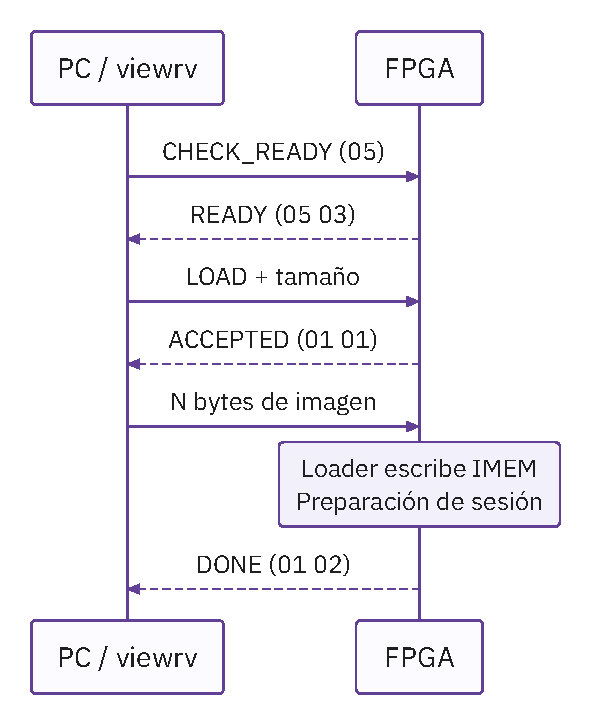
\includegraphics[width=0.42\textwidth]{secuencia-load.pdf}
  \caption{Secuencia normal de \code{LOAD}.}
  \label{fig:secuencia-load}
\end{figure}

\subsection{Secuencia de ejecución y observación}

Una vez cargada la imagen, la PC puede solicitar ejecución continua con
\code{RUN} o avanzar un ciclo con \code{STEP}. Un \code{RUN} aceptado recibe
primero \code{RUN/ACCEPTED}; cuando la sesión termina, la FPGA envía
\code{RUN/FINISHED} o \code{RUN/FAULT} junto con el snapshot final.

Cada \code{STEP} aceptado devuelve \code{STEP/DONE} y un snapshot posterior al
ciclo ejecutado. Durante la transmisión, la FPGA retiene el estado observado,
de modo que la respuesta describe un mismo instante de la sesión.

La tabla~\ref{tab:snapshot} muestra los campos del snapshot. Sus offsets se
cuentan desde el inicio del cuerpo, que sigue a la cabecera de dos bytes. El
cuerpo fijo ocupa 228 bytes y contiene, entre otros datos, el PC, los registros
arquitectónicos y el contenido de los registros interetapa.

Al final se agrega una entrada de cinco bytes por cada byte de DMEM escrito
durante la sesión: cuatro para la dirección y uno para el valor. Si $K$ es la
cantidad de entradas, la respuesta completa ocupa $230 + 5K$ bytes, incluida
la cabecera.

\begin{table}[H]
  \centering
  \small
  \begin{tabular}{lrl}
    \toprule
    \textbf{Campo} & \textbf{Offset} & \textbf{Bytes} \\
    \midrule
    \code{global_state} & 0 & 1 \\
    \code{image_valid} & 1 & 1 \\
    PC global & 2 & 4 \\
    \code{cycle_count} & 6 & 8 \\
    \code{fault_cause} & 14 & 1 \\
    \code{fault_pc} & 15 & 4 \\
    RF \code{x0..x31} & 19 & 128 \\
    \code{IF/ID} & 147 & 11 \\
    \code{ID/EX} & 158 & 30 \\
    \code{EX/MEM} & 188 & 20 \\
    \code{MEM/WB} & 208 & 15 \\
    \code{used_count} & 223 & 5 \\
    Lista de memoria & 228 & $5K$ \\
    \bottomrule
  \end{tabular}
  \caption{Estructura del snapshot de Debug. Los offsets del cuerpo se cuentan
  después de la cabecera de dos bytes.}
  \label{tab:snapshot}
\end{table}

\section{Cómo se observa el estado}

El snapshot permite examinar el estado del procesador después de un ciclo o al
finalizar una ejecución. Para construirlo, el serializador de la FPGA lee los
registros y la memoria definidos por el protocolo, mientras el estado de la
sesión permanece retenido. La aplicación recibe esos bytes y reconstruye:

\begin{itemize}
  \item el estado global de la sesión y la validez de la imagen;
  \item el PC y el contador de ciclos;
  \item la causa y el PC de fault, cuando corresponde;
  \item los 32 registros del banco;
  \item los 34 campos de los cuatro registros interetapa;
  \item la cantidad y la lista de bytes de DMEM escritos en la sesión.
\end{itemize}

Con esos datos, la GUI puede mostrar los registros, el contenido del pipeline,
la memoria utilizada y la línea de código asociada a una instrucción. La CLI
accede a la misma información y puede conservar los resultados en JSONL. El
mapa generado por el assembler permite relacionar los PC observados con el
código fuente de la imagen cargada.

Durante la depuración, la aplicación puede solicitar pasos sucesivos y examinar
cada snapshot para detectar coincidencias con los breakpoints configurados. La
observación corresponde a los datos recibidos de la FPGA; la aplicación
distingue esos datos de las interpretaciones que presenta al usuario.

Para que todos sus campos correspondan al mismo estado, la FPGA no admite otro
ciclo de CPU, una carga ni una preparación mientras se transmite el snapshot.
Si la respuesta se interrumpe, la PC descarta la captura parcial y conserva la
última que recibió completa, identificándola como anterior. La semántica
completa se consulta en
\doc{architecture/debug/debug_architecture.md}{Arquitectura de Debug} y en
\doc{protocol.md}{Protocolo UART}.
